% Options for packages loaded elsewhere
\PassOptionsToPackage{unicode}{hyperref}
\PassOptionsToPackage{hyphens}{url}
\documentclass[
]{article}
\usepackage{xcolor}
\usepackage[margin=1in]{geometry}
\usepackage{amsmath,amssymb}
\setcounter{secnumdepth}{-\maxdimen} % remove section numbering
\usepackage{iftex}
\ifPDFTeX
  \usepackage[T1]{fontenc}
  \usepackage[utf8]{inputenc}
  \usepackage{textcomp} % provide euro and other symbols
\else % if luatex or xetex
  \usepackage{unicode-math} % this also loads fontspec
  \defaultfontfeatures{Scale=MatchLowercase}
  \defaultfontfeatures[\rmfamily]{Ligatures=TeX,Scale=1}
\fi
\usepackage{lmodern}
\ifPDFTeX\else
  % xetex/luatex font selection
\fi
% Use upquote if available, for straight quotes in verbatim environments
\IfFileExists{upquote.sty}{\usepackage{upquote}}{}
\IfFileExists{microtype.sty}{% use microtype if available
  \usepackage[]{microtype}
  \UseMicrotypeSet[protrusion]{basicmath} % disable protrusion for tt fonts
}{}
\makeatletter
\@ifundefined{KOMAClassName}{% if non-KOMA class
  \IfFileExists{parskip.sty}{%
    \usepackage{parskip}
  }{% else
    \setlength{\parindent}{0pt}
    \setlength{\parskip}{6pt plus 2pt minus 1pt}}
}{% if KOMA class
  \KOMAoptions{parskip=half}}
\makeatother
\usepackage{color}
\usepackage{fancyvrb}
\newcommand{\VerbBar}{|}
\newcommand{\VERB}{\Verb[commandchars=\\\{\}]}
\DefineVerbatimEnvironment{Highlighting}{Verbatim}{commandchars=\\\{\}}
% Add ',fontsize=\small' for more characters per line
\usepackage{framed}
\definecolor{shadecolor}{RGB}{248,248,248}
\newenvironment{Shaded}{\begin{snugshade}}{\end{snugshade}}
\newcommand{\AlertTok}[1]{\textcolor[rgb]{0.94,0.16,0.16}{#1}}
\newcommand{\AnnotationTok}[1]{\textcolor[rgb]{0.56,0.35,0.01}{\textbf{\textit{#1}}}}
\newcommand{\AttributeTok}[1]{\textcolor[rgb]{0.13,0.29,0.53}{#1}}
\newcommand{\BaseNTok}[1]{\textcolor[rgb]{0.00,0.00,0.81}{#1}}
\newcommand{\BuiltInTok}[1]{#1}
\newcommand{\CharTok}[1]{\textcolor[rgb]{0.31,0.60,0.02}{#1}}
\newcommand{\CommentTok}[1]{\textcolor[rgb]{0.56,0.35,0.01}{\textit{#1}}}
\newcommand{\CommentVarTok}[1]{\textcolor[rgb]{0.56,0.35,0.01}{\textbf{\textit{#1}}}}
\newcommand{\ConstantTok}[1]{\textcolor[rgb]{0.56,0.35,0.01}{#1}}
\newcommand{\ControlFlowTok}[1]{\textcolor[rgb]{0.13,0.29,0.53}{\textbf{#1}}}
\newcommand{\DataTypeTok}[1]{\textcolor[rgb]{0.13,0.29,0.53}{#1}}
\newcommand{\DecValTok}[1]{\textcolor[rgb]{0.00,0.00,0.81}{#1}}
\newcommand{\DocumentationTok}[1]{\textcolor[rgb]{0.56,0.35,0.01}{\textbf{\textit{#1}}}}
\newcommand{\ErrorTok}[1]{\textcolor[rgb]{0.64,0.00,0.00}{\textbf{#1}}}
\newcommand{\ExtensionTok}[1]{#1}
\newcommand{\FloatTok}[1]{\textcolor[rgb]{0.00,0.00,0.81}{#1}}
\newcommand{\FunctionTok}[1]{\textcolor[rgb]{0.13,0.29,0.53}{\textbf{#1}}}
\newcommand{\ImportTok}[1]{#1}
\newcommand{\InformationTok}[1]{\textcolor[rgb]{0.56,0.35,0.01}{\textbf{\textit{#1}}}}
\newcommand{\KeywordTok}[1]{\textcolor[rgb]{0.13,0.29,0.53}{\textbf{#1}}}
\newcommand{\NormalTok}[1]{#1}
\newcommand{\OperatorTok}[1]{\textcolor[rgb]{0.81,0.36,0.00}{\textbf{#1}}}
\newcommand{\OtherTok}[1]{\textcolor[rgb]{0.56,0.35,0.01}{#1}}
\newcommand{\PreprocessorTok}[1]{\textcolor[rgb]{0.56,0.35,0.01}{\textit{#1}}}
\newcommand{\RegionMarkerTok}[1]{#1}
\newcommand{\SpecialCharTok}[1]{\textcolor[rgb]{0.81,0.36,0.00}{\textbf{#1}}}
\newcommand{\SpecialStringTok}[1]{\textcolor[rgb]{0.31,0.60,0.02}{#1}}
\newcommand{\StringTok}[1]{\textcolor[rgb]{0.31,0.60,0.02}{#1}}
\newcommand{\VariableTok}[1]{\textcolor[rgb]{0.00,0.00,0.00}{#1}}
\newcommand{\VerbatimStringTok}[1]{\textcolor[rgb]{0.31,0.60,0.02}{#1}}
\newcommand{\WarningTok}[1]{\textcolor[rgb]{0.56,0.35,0.01}{\textbf{\textit{#1}}}}
\usepackage{graphicx}
\makeatletter
\newsavebox\pandoc@box
\newcommand*\pandocbounded[1]{% scales image to fit in text height/width
  \sbox\pandoc@box{#1}%
  \Gscale@div\@tempa{\textheight}{\dimexpr\ht\pandoc@box+\dp\pandoc@box\relax}%
  \Gscale@div\@tempb{\linewidth}{\wd\pandoc@box}%
  \ifdim\@tempb\p@<\@tempa\p@\let\@tempa\@tempb\fi% select the smaller of both
  \ifdim\@tempa\p@<\p@\scalebox{\@tempa}{\usebox\pandoc@box}%
  \else\usebox{\pandoc@box}%
  \fi%
}
% Set default figure placement to htbp
\def\fps@figure{htbp}
\makeatother
\setlength{\emergencystretch}{3em} % prevent overfull lines
\providecommand{\tightlist}{%
  \setlength{\itemsep}{0pt}\setlength{\parskip}{0pt}}
\usepackage{bookmark}
\IfFileExists{xurl.sty}{\usepackage{xurl}}{} % add URL line breaks if available
\urlstyle{same}
\hypersetup{
  pdftitle={Week4hw},
  pdfauthor={Owen Hughes},
  hidelinks,
  pdfcreator={LaTeX via pandoc}}

\title{Week4hw}
\author{Owen Hughes}
\date{2025-10-22}

\begin{document}
\maketitle

\subsection{R Markdown}\label{r-markdown}

This is an R Markdown document. Markdown is a simple formatting syntax
for authoring HTML, PDF, and MS Word documents. For more details on
using R Markdown see \url{http://rmarkdown.rstudio.com}.

When you click the \textbf{Knit} button a document will be generated
that includes both content as well as the output of any embedded R code
chunks within the document. You can embed an R code chunk like this:

\begin{Shaded}
\begin{Highlighting}[]
\FunctionTok{summary}\NormalTok{(cars)}
\end{Highlighting}
\end{Shaded}

\begin{verbatim}
##      speed           dist       
##  Min.   : 4.0   Min.   :  2.00  
##  1st Qu.:12.0   1st Qu.: 26.00  
##  Median :15.0   Median : 36.00  
##  Mean   :15.4   Mean   : 42.98  
##  3rd Qu.:19.0   3rd Qu.: 56.00  
##  Max.   :25.0   Max.   :120.00
\end{verbatim}

\subsection{Including Plots}\label{including-plots}

You can also embed plots, for example:

\pandocbounded{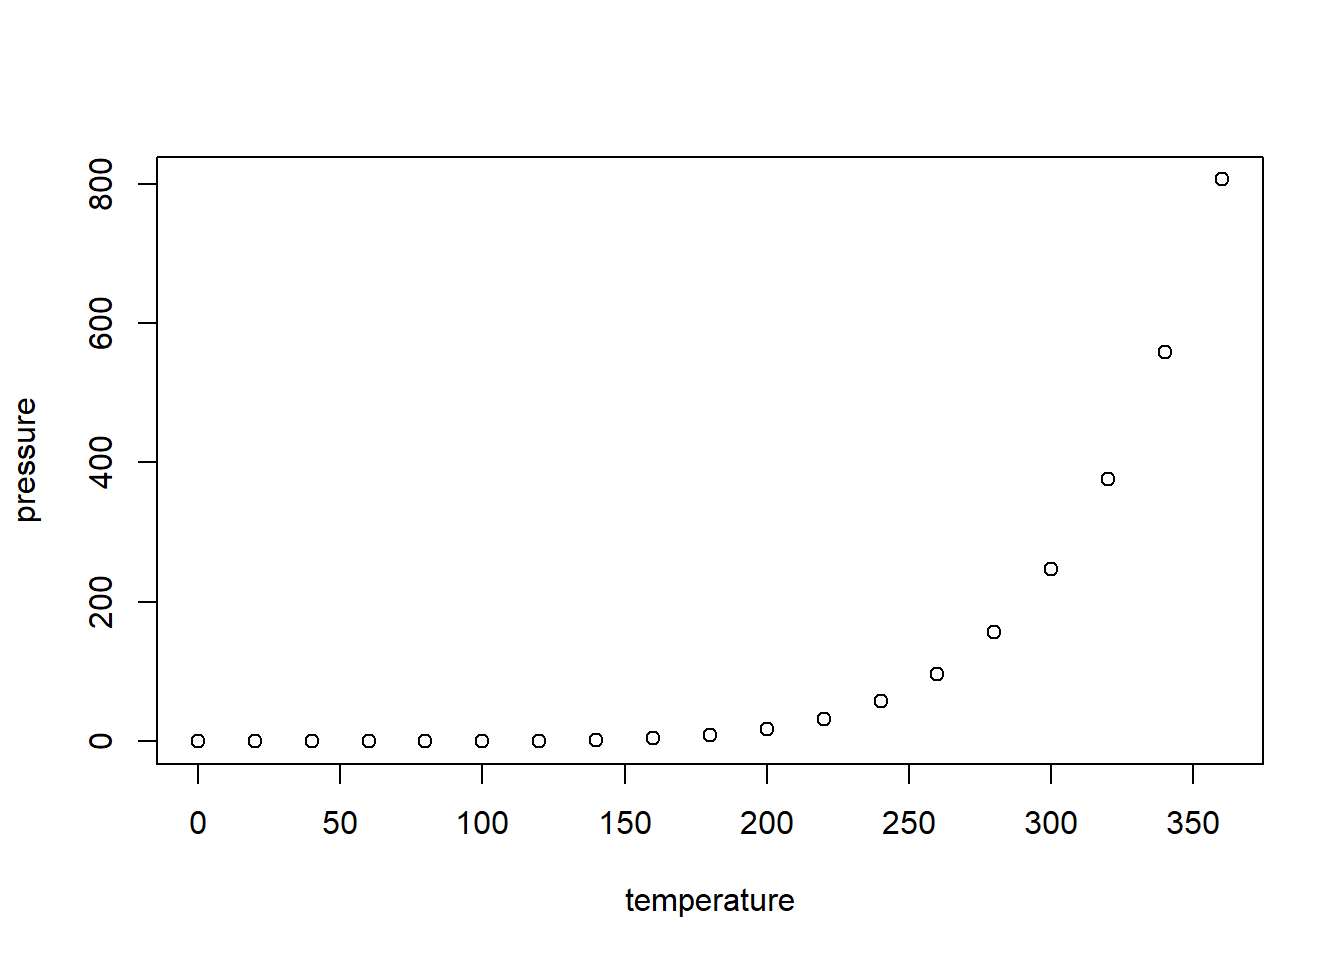
\includegraphics[keepaspectratio]{Week4hw_files/figure-latex/pressure-1.pdf}}

Note that the \texttt{echo\ =\ FALSE} parameter was added to the code
chunk to prevent printing of the R code that generated the plot.

\begin{Shaded}
\begin{Highlighting}[]
\FunctionTok{print}\NormalTok{(}\StringTok{\textquotesingle{}Okay!! I Want to Load the World Data and Gender Inequality Data, Make a New Column}
\StringTok{      Displaying the Difference Between 2010 and 2019, Save to GitHub, and Add my GitHub}
\StringTok{      URL to the spreadsheet\textquotesingle{}}\NormalTok{)}
\end{Highlighting}
\end{Shaded}

\begin{verbatim}
## [1] "Okay!! I Want to Load the World Data and Gender Inequality Data, Make a New Column\n      Displaying the Difference Between 2010 and 2019, Save to GitHub, and Add my GitHub\n      URL to the spreadsheet"
\end{verbatim}

\begin{Shaded}
\begin{Highlighting}[]
\FunctionTok{print}\NormalTok{(}\StringTok{\textquotesingle{}The First Step is to Load the Packeges that I Think I Might Need\textquotesingle{}}\NormalTok{)}
\end{Highlighting}
\end{Shaded}

\begin{verbatim}
## [1] "The First Step is to Load the Packeges that I Think I Might Need"
\end{verbatim}

\begin{Shaded}
\begin{Highlighting}[]
\FunctionTok{library}\NormalTok{(sf)}
\end{Highlighting}
\end{Shaded}

\begin{verbatim}
## Linking to GEOS 3.13.1, GDAL 3.11.0, PROJ 9.6.0; sf_use_s2() is TRUE
\end{verbatim}

\begin{Shaded}
\begin{Highlighting}[]
\FunctionTok{library}\NormalTok{(here)}
\end{Highlighting}
\end{Shaded}

\begin{verbatim}
## here() starts at C:/Users/Owen Hughes/Desktop/CASA/UCL_Work/GIS_Term1/GIS_Git_Projects/Week_4_hw/GIS
\end{verbatim}

\begin{Shaded}
\begin{Highlighting}[]
\FunctionTok{library}\NormalTok{(janitor)}
\end{Highlighting}
\end{Shaded}

\begin{verbatim}
## 
## Attaching package: 'janitor'
\end{verbatim}

\begin{verbatim}
## The following objects are masked from 'package:stats':
## 
##     chisq.test, fisher.test
\end{verbatim}

\begin{Shaded}
\begin{Highlighting}[]
\FunctionTok{library}\NormalTok{(tidyverse)}
\end{Highlighting}
\end{Shaded}

\begin{verbatim}
## -- Attaching core tidyverse packages ------------------------ tidyverse 2.0.0 --
## v dplyr     1.1.4     v readr     2.1.5
## v forcats   1.0.1     v stringr   1.5.2
## v ggplot2   4.0.0     v tibble    3.3.0
## v lubridate 1.9.4     v tidyr     1.3.1
## v purrr     1.1.0
\end{verbatim}

\begin{verbatim}
## -- Conflicts ------------------------------------------ tidyverse_conflicts() --
## x dplyr::filter() masks stats::filter()
## x dplyr::lag()    masks stats::lag()
## i Use the conflicted package (<http://conflicted.r-lib.org/>) to force all conflicts to become errors
\end{verbatim}

\begin{Shaded}
\begin{Highlighting}[]
\FunctionTok{library}\NormalTok{(ggplot2)}
\end{Highlighting}
\end{Shaded}

\begin{Shaded}
\begin{Highlighting}[]
\FunctionTok{print}\NormalTok{(}\StringTok{"Let\textquotesingle{}s read these files"}\NormalTok{)}
\end{Highlighting}
\end{Shaded}

\begin{verbatim}
## [1] "Let's read these files"
\end{verbatim}

\begin{Shaded}
\begin{Highlighting}[]
\NormalTok{gen\_ineq }\OtherTok{\textless{}{-}} \FunctionTok{st\_read}\NormalTok{(}\FunctionTok{here}\NormalTok{(}\StringTok{\textquotesingle{}HDR25\_Composite\_indices\_complete\_time\_series.csv\textquotesingle{}}\NormalTok{))}
\end{Highlighting}
\end{Shaded}

\begin{verbatim}
## Reading layer `HDR25_Composite_indices_complete_time_series' from data source 
##   `C:\Users\Owen Hughes\Desktop\CASA\UCL_Work\GIS_Term1\GIS_Git_Projects\Week_4_hw\GIS\HDR25_Composite_indices_complete_time_series.csv' 
##   using driver `CSV'
\end{verbatim}

\begin{verbatim}
## Warning: no simple feature geometries present: returning a data.frame or tbl_df
\end{verbatim}

\begin{Shaded}
\begin{Highlighting}[]
\NormalTok{paices }\OtherTok{\textless{}{-}} \FunctionTok{st\_read}\NormalTok{(}\FunctionTok{here}\NormalTok{(}\StringTok{\textquotesingle{}World\_Countries/World\_Countries\_Generalized.shp\textquotesingle{}}\NormalTok{))}
\end{Highlighting}
\end{Shaded}

\begin{verbatim}
## Reading layer `World_Countries_Generalized' from data source 
##   `C:\Users\Owen Hughes\Desktop\CASA\UCL_Work\GIS_Term1\GIS_Git_Projects\Week_4_hw\GIS\World_Countries\World_Countries_Generalized.shp' 
##   using driver `ESRI Shapefile'
## Simple feature collection with 251 features and 4 fields
## Geometry type: MULTIPOLYGON
## Dimension:     XY
## Bounding box:  xmin: -20037510 ymin: -30240970 xmax: 20037510 ymax: 18418390
## Projected CRS: WGS 84 / Pseudo-Mercator
\end{verbatim}

\begin{Shaded}
\begin{Highlighting}[]
\FunctionTok{print}\NormalTok{(}\StringTok{"Let\textquotesingle{}s inspect the data"}\NormalTok{)}
\end{Highlighting}
\end{Shaded}

\begin{verbatim}
## [1] "Let's inspect the data"
\end{verbatim}

\begin{Shaded}
\begin{Highlighting}[]
\FunctionTok{view}\NormalTok{(gen\_ineq)}
\FunctionTok{plot}\NormalTok{(paices)}
\end{Highlighting}
\end{Shaded}

\pandocbounded{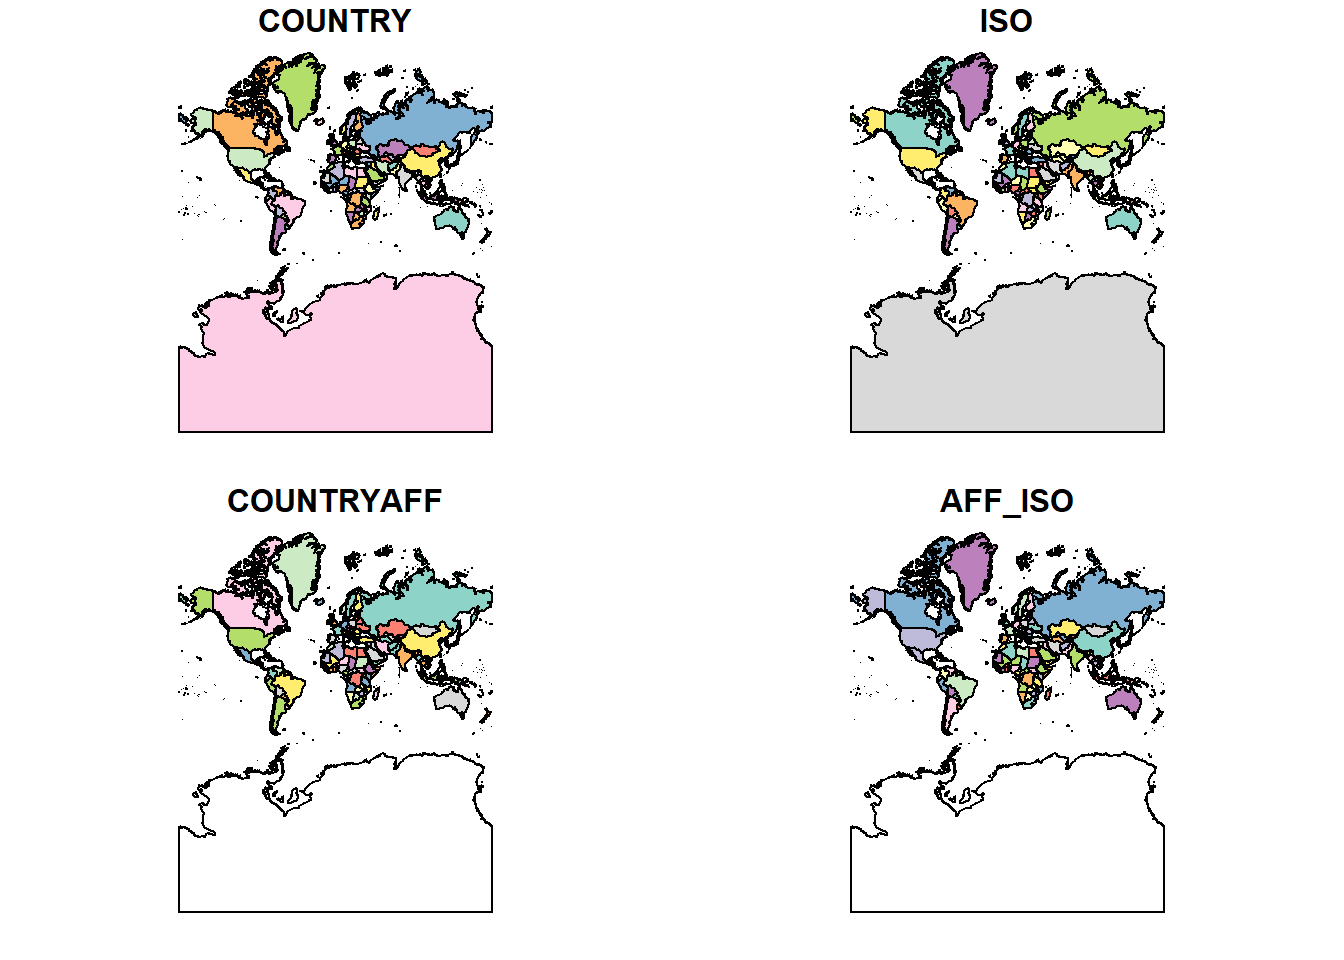
\includegraphics[keepaspectratio]{Week4hw_files/figure-latex/unnamed-chunk-4-1.pdf}}

\begin{Shaded}
\begin{Highlighting}[]
\FunctionTok{print}\NormalTok{(}\StringTok{\textquotesingle{}Okay, I see that in the paices data I want to remove antarctica because it is massive}
\StringTok{      and in the gen\_ineq I want to select only the columns containing country name,}
\StringTok{      gii\_2010 and gii\_2019\textquotesingle{}}\NormalTok{)}
\end{Highlighting}
\end{Shaded}

\begin{verbatim}
## [1] "Okay, I see that in the paices data I want to remove antarctica because it is massive\n      and in the gen_ineq I want to select only the columns containing country name,\n      gii_2010 and gii_2019"
\end{verbatim}

\begin{Shaded}
\begin{Highlighting}[]
\NormalTok{solo\_paices }\OtherTok{\textless{}{-}}\NormalTok{ paices }\SpecialCharTok{\%\textgreater{}\%} \FunctionTok{filter}\NormalTok{(COUNTRYAFF }\SpecialCharTok{!=} \StringTok{\textquotesingle{}AQ\textquotesingle{}}\NormalTok{)}
\FunctionTok{view}\NormalTok{(solo\_paices)}

\NormalTok{gen\_ineq2 }\OtherTok{\textless{}{-}}\NormalTok{ gen\_ineq }\SpecialCharTok{\%\textgreater{}\%} 
  \FunctionTok{select}\NormalTok{(}\FunctionTok{any\_of}\NormalTok{(}\FunctionTok{c}\NormalTok{(}\StringTok{\textquotesingle{}country\textquotesingle{}}\NormalTok{, }\StringTok{\textquotesingle{}gii\_2010\textquotesingle{}}\NormalTok{, }\StringTok{\textquotesingle{}gii\_2019\textquotesingle{}}\NormalTok{, }\StringTok{\textquotesingle{}iso3\textquotesingle{}}\NormalTok{))) }
\FunctionTok{view}\NormalTok{(gen\_ineq2)}
\FunctionTok{plot}\NormalTok{(solo\_paices)}
\end{Highlighting}
\end{Shaded}

\pandocbounded{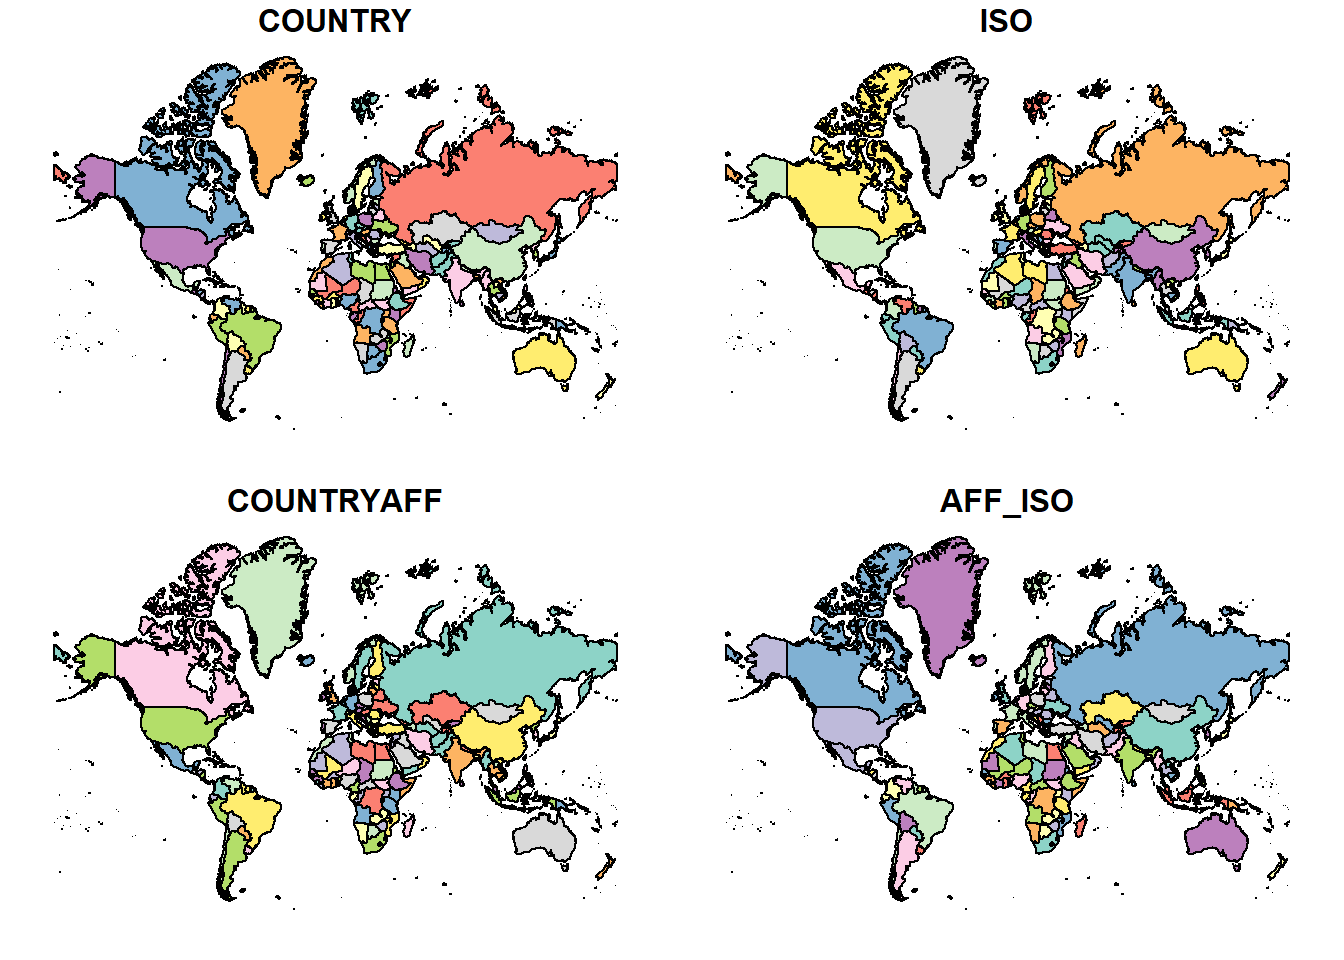
\includegraphics[keepaspectratio]{Week4hw_files/figure-latex/unnamed-chunk-5-1.pdf}}

\begin{Shaded}
\begin{Highlighting}[]
\FunctionTok{print}\NormalTok{(}\StringTok{"Now I want to take the difference of the 2010 and 2019 gender inequality values}
\StringTok{      A quick inspection of the table shows that the 2010 values are generally higher so }
\StringTok{      I will do (2010 value {-} 2019 value)"}\NormalTok{)}
\end{Highlighting}
\end{Shaded}

\begin{verbatim}
## [1] "Now I want to take the difference of the 2010 and 2019 gender inequality values\n      A quick inspection of the table shows that the 2010 values are generally higher so \n      I will do (2010 value - 2019 value)"
\end{verbatim}

\begin{Shaded}
\begin{Highlighting}[]
\NormalTok{gen\_ineq\_diff }\OtherTok{\textless{}{-}}\NormalTok{ gen\_ineq2 }\SpecialCharTok{\%\textgreater{}\%}
  \FunctionTok{mutate}\NormalTok{(}
    \AttributeTok{gii\_2010 =} \FunctionTok{as.numeric}\NormalTok{(gii\_2010),}
    \AttributeTok{gii\_2019 =} \FunctionTok{as.numeric}\NormalTok{(gii\_2019),}
    \AttributeTok{difference =}\NormalTok{ gii\_2010 }\SpecialCharTok{{-}}\NormalTok{ gii\_2019)}
\FunctionTok{view}\NormalTok{(gen\_ineq\_diff)}
\end{Highlighting}
\end{Shaded}

\begin{Shaded}
\begin{Highlighting}[]
\FunctionTok{print}\NormalTok{(}\StringTok{"Alrighty it looks like imma have to work some magic to attain a key field in both}
\StringTok{      datasets to execute a join. Let\textquotesingle{}s investigate the countrycode package that Andy suggests"}\NormalTok{)}
\end{Highlighting}
\end{Shaded}

\begin{verbatim}
## [1] "Alrighty it looks like imma have to work some magic to attain a key field in both\n      datasets to execute a join. Let's investigate the countrycode package that Andy suggests"
\end{verbatim}

\begin{Shaded}
\begin{Highlighting}[]
\FunctionTok{print}\NormalTok{(}\StringTok{"Run this code [install.packages(\textquotesingle{}countrycode\textquotesingle{})] in the console to install the package"}\NormalTok{)}
\end{Highlighting}
\end{Shaded}

\begin{verbatim}
## [1] "Run this code [install.packages('countrycode')] in the console to install the package"
\end{verbatim}

\begin{Shaded}
\begin{Highlighting}[]
\FunctionTok{library}\NormalTok{(countrycode)}

\FunctionTok{print}\NormalTok{(}\StringTok{\textquotesingle{}I am going to change the ISO3 values in gen\_ineq\_diff into ISO2 values similar to those in}
\StringTok{      the solo\_paices data\textquotesingle{}}\NormalTok{)}
\end{Highlighting}
\end{Shaded}

\begin{verbatim}
## [1] "I am going to change the ISO3 values in gen_ineq_diff into ISO2 values similar to those in\n      the solo_paices data"
\end{verbatim}

\begin{Shaded}
\begin{Highlighting}[]
\NormalTok{gen\_ineq\_diff }\OtherTok{\textless{}{-}}\NormalTok{ gen\_ineq\_diff }\SpecialCharTok{\%\textgreater{}\%}
  \FunctionTok{mutate}\NormalTok{(}\AttributeTok{iso2 =} \FunctionTok{countrycode}\NormalTok{(iso3, }\AttributeTok{origin =} \StringTok{\textquotesingle{}iso3c\textquotesingle{}}\NormalTok{, }\AttributeTok{destination =} \StringTok{\textquotesingle{}iso2c\textquotesingle{}}\NormalTok{))}
\end{Highlighting}
\end{Shaded}

\begin{verbatim}
## Warning: There was 1 warning in `mutate()`.
## i In argument: `iso2 = countrycode(iso3, origin = "iso3c", destination =
##   "iso2c")`.
## Caused by warning:
## ! Some values were not matched unambiguously: ZZA.VHHD, ZZB.HHD, ZZC.MHD, ZZD.LHD, ZZE.AS, ZZF.EAP, ZZG.ECA, ZZH.LAC, ZZI.SA, ZZJ.SSA, ZZK.WORLD
\end{verbatim}

\begin{Shaded}
\begin{Highlighting}[]
\FunctionTok{view}\NormalTok{(gen\_ineq\_diff)}
\end{Highlighting}
\end{Shaded}

\begin{Shaded}
\begin{Highlighting}[]
\FunctionTok{print}\NormalTok{(}\StringTok{"Badabing badaboom let\textquotesingle{}s get crackalackin with the last bit of code now. I want to join}
\StringTok{      the two datasets with the new columns that I have made!!"}\NormalTok{)}
\end{Highlighting}
\end{Shaded}

\begin{verbatim}
## [1] "Badabing badaboom let's get crackalackin with the last bit of code now. I want to join\n      the two datasets with the new columns that I have made!!"
\end{verbatim}

\begin{Shaded}
\begin{Highlighting}[]
\NormalTok{gen\_ineq\_paices }\OtherTok{\textless{}{-}} \FunctionTok{left\_join}\NormalTok{(solo\_paices, gen\_ineq\_diff, }\AttributeTok{by =} \FunctionTok{c}\NormalTok{(}\StringTok{\textquotesingle{}ISO\textquotesingle{}} \OtherTok{=} \StringTok{\textquotesingle{}iso2\textquotesingle{}}\NormalTok{))}
\FunctionTok{view}\NormalTok{(gen\_ineq\_paices)}
\end{Highlighting}
\end{Shaded}

\begin{Shaded}
\begin{Highlighting}[]
\FunctionTok{print}\NormalTok{(}\StringTok{"SPECTACULAR! Now I want to clean up the final dataset so it is more easy to read"}\NormalTok{)}
\end{Highlighting}
\end{Shaded}

\begin{verbatim}
## [1] "SPECTACULAR! Now I want to clean up the final dataset so it is more easy to read"
\end{verbatim}

\begin{Shaded}
\begin{Highlighting}[]
\NormalTok{gen\_ineq\_paices2 }\OtherTok{\textless{}{-}}\NormalTok{ gen\_ineq\_paices }\SpecialCharTok{\%\textgreater{}\%}
  \FunctionTok{select}\NormalTok{(}\FunctionTok{any\_of}\NormalTok{(}\FunctionTok{c}\NormalTok{(}\StringTok{\textquotesingle{}COUNTRY\textquotesingle{}}\NormalTok{, }\StringTok{\textquotesingle{}gii\_2010\textquotesingle{}}\NormalTok{, }\StringTok{\textquotesingle{}gii\_2019\textquotesingle{}}\NormalTok{, }\StringTok{\textquotesingle{}difference\textquotesingle{}}\NormalTok{, }\StringTok{\textquotesingle{}iso2\textquotesingle{}}\NormalTok{, }
                  \StringTok{\textquotesingle{}geometry\textquotesingle{}}\NormalTok{))) }\SpecialCharTok{\%\textgreater{}\%}
  \FunctionTok{clean\_names}\NormalTok{()}
\FunctionTok{view}\NormalTok{(gen\_ineq\_paices2)}
\end{Highlighting}
\end{Shaded}

\begin{Shaded}
\begin{Highlighting}[]
\FunctionTok{print}\NormalTok{(}\StringTok{"Alright I just realized that there are regions included in this data like sub{-}saharan africa,}
\StringTok{      let\textquotesingle{}s remove those. I am going to filter all the areas without and ISO2 value"}\NormalTok{)}
\end{Highlighting}
\end{Shaded}

\begin{verbatim}
## [1] "Alright I just realized that there are regions included in this data like sub-saharan africa,\n      let's remove those. I am going to filter all the areas without and ISO2 value"
\end{verbatim}

\begin{Shaded}
\begin{Highlighting}[]
\FunctionTok{print}\NormalTok{(}\StringTok{\textquotesingle{}gen\_ineq\_paices2 \textless{}{-} gen\_ineq\_paices2 \%\textgreater{}\%}
\StringTok{  filter(!is.na(iso2))}
\StringTok{view(gen\_ineq\_paices2)}
\StringTok{plot(st\_geometry(gen\_ineq\_paices2))\textquotesingle{}}\NormalTok{)}
\end{Highlighting}
\end{Shaded}

\begin{verbatim}
## [1] "gen_ineq_paices2 <- gen_ineq_paices2 %>%\n  filter(!is.na(iso2))\nview(gen_ineq_paices2)\nplot(st_geometry(gen_ineq_paices2))"
\end{verbatim}

\begin{Shaded}
\begin{Highlighting}[]
\DocumentationTok{\#\# I switched the order of the join dataframes to mainetain the geometry so this is pointless}
\DocumentationTok{\#\# good to know tho}
\end{Highlighting}
\end{Shaded}

\begin{Shaded}
\begin{Highlighting}[]
\FunctionTok{plot}\NormalTok{(gen\_ineq\_paices2)}
\end{Highlighting}
\end{Shaded}

\pandocbounded{\includegraphics[keepaspectratio]{Week4hw_files/figure-latex/unnamed-chunk-11-1.pdf}}

\begin{Shaded}
\begin{Highlighting}[]
\FunctionTok{print}\NormalTok{(}\StringTok{\textquotesingle{}Alrighty I want to make a choropleth map of the difference in gender inquality by country!\textquotesingle{}}\NormalTok{)}
\end{Highlighting}
\end{Shaded}

\begin{verbatim}
## [1] "Alrighty I want to make a choropleth map of the difference in gender inquality by country!"
\end{verbatim}

\begin{Shaded}
\begin{Highlighting}[]
\NormalTok{gen\_ineq\_map }\OtherTok{\textless{}{-}} \FunctionTok{ggplot}\NormalTok{(gen\_ineq\_paices2) }\SpecialCharTok{+}
  \FunctionTok{geom\_sf}\NormalTok{(}\FunctionTok{aes}\NormalTok{(}\AttributeTok{fill =}\NormalTok{ difference), }\AttributeTok{color =} \StringTok{\textquotesingle{}\#F0EAD6\textquotesingle{}}\NormalTok{, }\AttributeTok{size =} \FloatTok{0.1}\NormalTok{) }\SpecialCharTok{+}
  \FunctionTok{scale\_fill\_gradient2}\NormalTok{(}
    \AttributeTok{low =} \StringTok{\textquotesingle{}\#3c0008\textquotesingle{}}\NormalTok{, }\AttributeTok{mid =} \StringTok{\textquotesingle{}\#cc7070\textquotesingle{}}\NormalTok{, }\AttributeTok{high =} \StringTok{\textquotesingle{}\#ff69b4\textquotesingle{}}\NormalTok{,}
    \AttributeTok{midpoint =} \FloatTok{0.1}\NormalTok{,}
    \AttributeTok{name =} \StringTok{"[2010{-}2019] GII"}
\NormalTok{  ) }\SpecialCharTok{+}
  \FunctionTok{theme\_minimal}\NormalTok{() }\SpecialCharTok{+}
  \FunctionTok{labs}\NormalTok{(}
    \AttributeTok{title =} \StringTok{\textquotesingle{}Difference in Gender Inequality Between 2019 and 2010\textquotesingle{}}\NormalTok{,}
    \AttributeTok{subtitle =} \StringTok{\textquotesingle{}Higher Numbers = Gender Equality Gains\textquotesingle{}}\NormalTok{,}
\NormalTok{  )}

\FunctionTok{plot}\NormalTok{(gen\_ineq\_map)}
\end{Highlighting}
\end{Shaded}

\pandocbounded{\includegraphics[keepaspectratio]{Week4hw_files/figure-latex/unnamed-chunk-12-1.pdf}}

\end{document}
